\section{Test-circuit results}
\label{sec:circuit}

The parity checker is simulated in SPICE as one 112-transistor netlist for all 256 input vectors at the same 200 corners (51,200 cases). The ML prediction propagates the Boolean input vector through the 28 NAND2 gates, looks up the NAND2 gate prediction for the resulting input pair at that corner, and sums the 28 values. Node voltages measured in the full circuit are not used. Table~\ref{tab:circ} gives the metrics (first two rows) and Figure~\ref{fig:cparity} the parity plot.

\begin{table}[H]
\centering
\small
\caption{Test-circuit results over all 256 input vectors at 200 corners. The last two rows are diagnostics that split the error (Section~\ref{sec:err}); the reference is the first-named quantity.}
\label{tab:circ}
\resizebox{\ifdim\width>\linewidth\linewidth\else\width\fi}{!}{%
\begin{tabular}{p{4.6cm}rrrrrr}
\toprule
Comparison & Reference median (nA) & Predicted median (nA) & Bias (nA) & Median err. (\%) & p95 err. (\%) & Mean acc. (\%) \\
\midrule
Gates, all 18 cases (3,600 rows) & 138.0 & 138.1 & -0.282 & 0.256 & 1.116 & 99.64 \\
Parity checker, ML vs full SPICE (51,200 rows) & 3616.1 & 3601.1 & -13.461 & 0.423 & 1.214 & 99.49 \\
Standalone SPICE gate sum vs full SPICE & 3616.1 & 3599.3 & -19.152 & 0.226 & 1.131 & 99.64 \\
ML vs standalone SPICE gate sum & 3599.3 & 3601.1 & +5.691 & 0.222 & 0.719 & 99.73 \\
\bottomrule
\end{tabular}%
}
\end{table}


\begin{figure}[H]
\centering
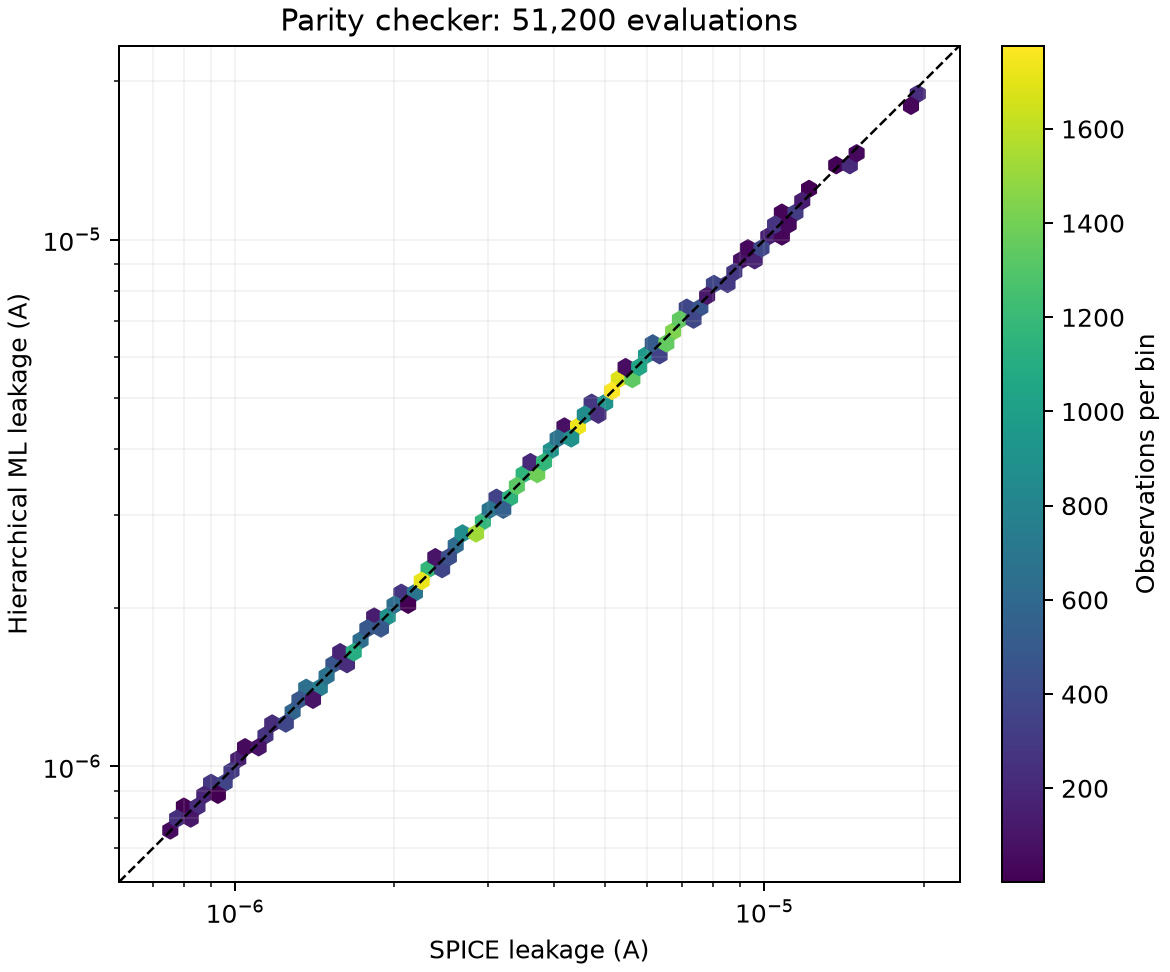
\includegraphics[width=0.6\linewidth]{figures/circuit_parity.png}
\caption{ML against SPICE leakage for all 51,200 circuit simulations (log axes).}
\label{fig:cparity}
\end{figure}

\textbf{Comparison with the gate level.} The circuit mean accuracy is 99.49\%, slightly lower than the gate-level 99.64\%, and the target of 99\% is met. The median error rises from 0.256\% to 0.423\% and the 95th percentile from 1.116\% to 1.214\%. The signed bias is $-0.165$\% (gates $-0.013$\%): the circuit is under-predicted on average. This is the expected direction. The circuit prediction assumes that every gate input is exactly at 0 or $V_{DD}$ and ignores loading between gates. The two diagnostic rows in Table~\ref{tab:circ} show where the extra error comes from. The standalone-gate sum is an evaluation-only diagnostic: it adds the true standalone SPICE gate leakages for the same Boolean states. It quantifies the error introduced by ideal-rail inputs and ignored inter-gate loading even if the transistor surrogate were perfect, and it is never substituted for an ML prediction. Summing the true standalone gate leakages (a perfect gate model) already gives a median error of 0.226\% and a mean accuracy of 99.64\% against the full circuit. The ML model differs from that sum by a median of 0.222\%. Thus the ideal-gate composition and the ML gate predictions each contribute a median error of about 0.22\%, and the two errors partly offset each other on average (bias $-0.30$\% for the composition and $+0.13$\% for ML against the standalone sum; Section~\ref{sec:err}). The circuit's 95th-percentile error stays near the gate-level one. The circuit error does not grow with its size, because the error of the ML sum relative to the standalone sum is a leakage-weighted average of the gate errors, and gate errors of opposite sign partly cancel.

\textbf{Per input vector.} The 256 vectors have similar accuracy. The median error is 0.38\% for the all-zero input, rises with the number of 1 bits and is 0.48\% for the all-one input (the highest). The mean accuracy over corners ranges from 99.43\% to 99.55\%, so every vector exceeds 99\%. The complete table is in \texttt{results/circuit\_metrics\_by\_vector.csv}.
